\documentclass{article}
\usepackage[utf8]{inputenc}
\usepackage{amsmath}
\usepackage{graphicx}

\title{Assignment 7}
\author{Swapnil Sirsat}
\date{January 2021}

\begin{document}

\maketitle

\section*{Question}
Draw a circle of radius \textbf{3} units. Take two points
\textbf{P} and \textbf{Q} on one of its extended diameter each
at a distance of \textbf{7} units from its centre. Draw
tangents to the circle from these two points \textbf{P}
and \textbf{Q}.
\section*{Answer}
Taking the center of the circle at (0,0)
\begin{gather*}
    O = (0,0)
\end{gather*}
Taking the diameter of the circle lie on the X axis \\
the extended diameter \textbf{PQ} would be
\begin{gather*}
    P = (-7,0)\\
    Q = (7,0)
\end{gather*}
now, constructing circles with the mid point of \textbf{OP} and \textbf{OQ} as centers and  \textbf{OP} and \textbf{OQ} as diameters respectively we obtain circle R and S as coordinates
\begin{gather*}
    R = (-3.5,0)\\
    S = (3.5,0)
\end{gather*}
the intersection points of Circle \textbf{R(-3.5,0)} and \textbf{S(-3.5,0)} with \textbf{O(0,0)} would be the points of contact of tangents through P and Q respectively
\\ joining this points we would obtain the asked tangents.
\newpage
below is the constructed figure.
\begin{figure}[h!]
    \centering
    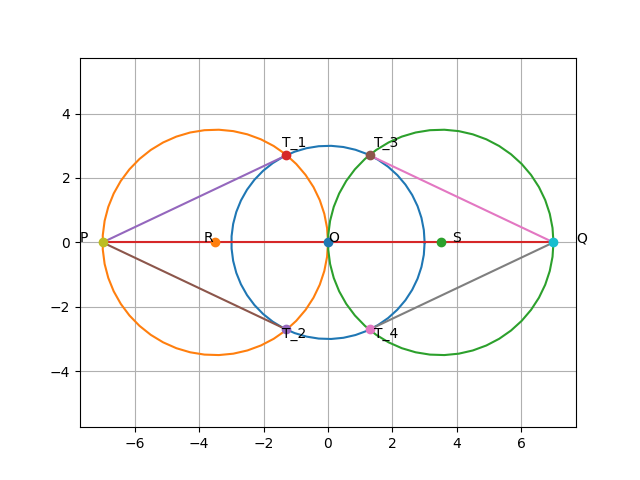
\includegraphics{Figure_1.png}
    \caption{Python output}
    \label{fig:my_label}
\end{figure}

\end{document}
